%% Copyright (c) 2015-2019, RTE (http://www.rte-france.com)
%% See AUTHORS.txt
%% All rights reserved.
%% This Source Code Form is subject to the terms of the Mozilla Public
%% License, v. 2.0. If a copy of the MPL was not distributed with this
%% file, you can obtain one at http://mozilla.org/MPL/2.0/.
%% SPDX-License-Identifier: MPL-2.0
%%
%% This file is part of Dynawo, a hybrid C++/Modelica open source time domain simulation tool for power systems.
\documentclass[a4paper, 12pt]{report}
%% Except where otherwise noted, content in this documentation is Copyright (c)
%% 2015-2019, RTE (http://www.rte-france.com) and licensed under a
%% CC-BY-4.0 (https://creativecommons.org/licenses/by/4.0/)
%% license. All rights reserved.

% Latin Modern fam­ily of fonts
\usepackage{lmodern}

\usepackage[english]{babel}

% specify encoding
\usepackage[utf8]{inputenc} % input
\usepackage[T1]{fontenc} % output

% Document structure setup
\usepackage{titlesec} % To change chapter format
\setcounter{tocdepth}{3} % Add subsubsection in Content
\setcounter{secnumdepth}{3} % Add numbering for subsubsection
\setlength{\parindent}{0pt} % No paragraph indentation

% Change title format for chapter
\titleformat{\chapter}{\Huge\bf}{\thechapter}{20pt}{\Huge\bf}

% To add links on page number in Content and hide red rectangle on links
\usepackage[hidelinks, linktoc=all]{hyperref}
\usepackage[nottoc]{tocbibind}  % To add biblio in table of content
\usepackage{textcomp} % For single quote
\usepackage{url} % Allow linebreaks in \url command
\usepackage{listings} % To add code samples

% Default listings parameters
\lstset
{
  aboveskip={1\baselineskip}, % a bit of space above
  backgroundcolor=\color{shadecolor}, % choose the background color
  basicstyle={\ttfamily\footnotesize}, % use font and smaller size \small \footnotesize
  breakatwhitespace=true, % sets if automatic breaks should only happen at whitespace
  breaklines=true, % sets automatic line breaking
  columns=fixed, % nice spacing -> fixed / flexible
  mathescape=false, % escape to latex false
  numbers=left, % where to put the line-numbers
  numberstyle=\tiny\color{gray}, % the style that is used for the line-numbers
  showstringspaces=false, % do not emphasize spaces in strings
  tabsize=4, % number of spaces of a TAB
  texcl=false, % activates or deactivates LaTeX comment lines
  upquote=true % upright quotes
}

% Avoid numbering starting at each chapter for figures
\usepackage{chngcntr}
\counterwithout{figure}{chapter}

\usepackage{tikz} % macro pack­age for cre­at­ing graph­ics
\usepackage{pgfplots} % draws func­tion plots (based on pgf/tikz)

\usepackage{algorithm} % Add algorithms
\usepackage[noend]{algpseudocode} %  all end ... lines are omitted in algos

\usepackage{amsmath} % Add math­e­mat­i­cal fea­tures
\usepackage{schemabloc} % Add block diagram library (french one)

\usepackage{adjustbox} % Add box for flowchart

\usepackage{booktabs} % for toprule and midrule in tables

\usepackage{tabularx}

\usepackage[nolist]{acronym} % don’t write the list of acronyms.
% Acronyms list
\begin{acronym}
\acro{BDF}{Backward Differentiation Formula}
\acro{BE}{Backward Euler}
\acro{DAE}{Differential Algebraic Equations}
\acro{IDA}{Implicit Differential-Algebraic solver}
\acro{LLNL}{Lawrence Livermore National Lab}
\acro{KINSOL}{Krylov Inexact Newton SOLver}
\acro{NR}{Newton-Raphson}
\acro{PLL}{Phase-Locked Loop}
\acro{SVC}{Static Var Compensator}
\acro{SUNDIALS}{SUite of Nonlinear and DIfferential/ALgebraic equation Solvers}
\acro{WECC}{Western Electricity Coordinating Council}
\end{acronym}

% Syntax highlight
%% Except where otherwise noted, content in this documentation is Copyright (c)
%% 2015-2019, RTE (http://www.rte-france.com) and licensed under a
%% CC-BY-4.0 (https://creativecommons.org/licenses/by/4.0/)
%% license. All rights reserved.

\usepackage{color}

\definecolor{blue}{rgb}{0,0,1}
\definecolor{lightblue}{rgb}{.3,.5,1}
\definecolor{darkblue}{rgb}{0,0,.4}
\definecolor{red}{rgb}{1,0,0}
\definecolor{darkred}{rgb}{.56,0,0}
\definecolor{pink}{rgb}{.933,0,.933}
\definecolor{purple}{rgb}{0.58,0,0.82}
\definecolor{green}{rgb}{0.133,0.545,0.133}
\definecolor{darkgreen}{rgb}{0,.4,0}
\definecolor{gray}{rgb}{.3,.3,.3}
\definecolor{darkgray}{rgb}{.2,.2,.2}
\definecolor{shadecolor}{gray}{0.925}

% **********************************************************************************
% Syntax : Bash (bash)
% **********************************************************************************

\lstdefinelanguage{bash}
{
  keywordstyle=\color{blue},
  morekeywords={
    cd,
    export,
    source},
  numbers=none,
  deletekeywords={jobs}
}

% **********************************************************************************
% Syntax : XML
% **********************************************************************************

\lstdefinelanguage{XML}
{
  morestring=[s][\color{purple}]{"}{"},
  morecomment=[s][\color{green}]{<?}{?>},
  morecomment=[s][\color{green}]{<!--}{-->},
  stringstyle=\color{black},
  identifierstyle=\color{blue},
  keywordstyle=\color{red},
  morekeywords={
    xmlns,
    xsi,
    noNamespaceSchemaLocation,
    type,
    source,
    target,
    version,
    tool,
    transRef,
    roleRef,
    objective,
    eventually}
}

% **********************************************************************************
% Syntax : Modelica (modelica)
% **********************************************************************************
\lstdefinelanguage{Modelica}{
  alsoletter={...},
  morekeywords=[1]{ % types
      Boolean,
      Integer,
      Real},
  keywordstyle=[1]\color{red},
  morekeywords=[2]{ % keywords
    algorithm,
    and,
    annotation,
    assert,
    block,
    class,
    connector,
    constant,
    discrete,
    else,
    elseif,
    elsewhen,
    end,
    equation,
    exit,
    extends,
    external,
    false,
    final,
    flow,
    for,
    function,
    if,
    in,
    inner,
    input,
    import,
    loop,
    model,
    nondiscrete,
    not,
    or,
    outer,
    output,
    package,
    parameter,
    public,
    protected,
    record,
    redeclare,
    replaceable,
    return,
    size,
    terminate,
    then,
    true,
    type,
    when,
    while},
  keywordstyle=[2]\color{darkred},
  morekeywords=[3]{ % functions
    abs,
    acos,
    asin,
    atan,
    atan2,
    Complex,
    connect,
    conj,
    cos,
    cosh,
    cross,
    der,
    edge,
    exp,
    fromPolar,
    imag,
    noEvent,
    pre,
    sign,
    sin,
    sinh,
    sqrt,
    tan,
    tanh},
  keywordstyle=[3]\color{blue},
  morecomment=[l][\color{green}]{//}, % comments
  morecomment=[s][\color{green}]{/*}{*/}, % comments
  morestring=[b][\color{pink}]{'}, % strings
  morestring=[b][\color{pink}]{"}, % strings
}


\usepackage{xspace} % Define typography
\usepackage{dirtree}
\newcommand{\Dynawo}[0]{Dyna$\omega$o\xspace}

\begin{document}
\chapter*{Three-converter system with three different types of Grid Forming Converters}
\section*{Test case description}
The studied test case is a simple system with three converters and one fully resistive load, as depicted in Fig.~\ref{ThreeConv}.
\begin{figure}[H]
\begin{center}
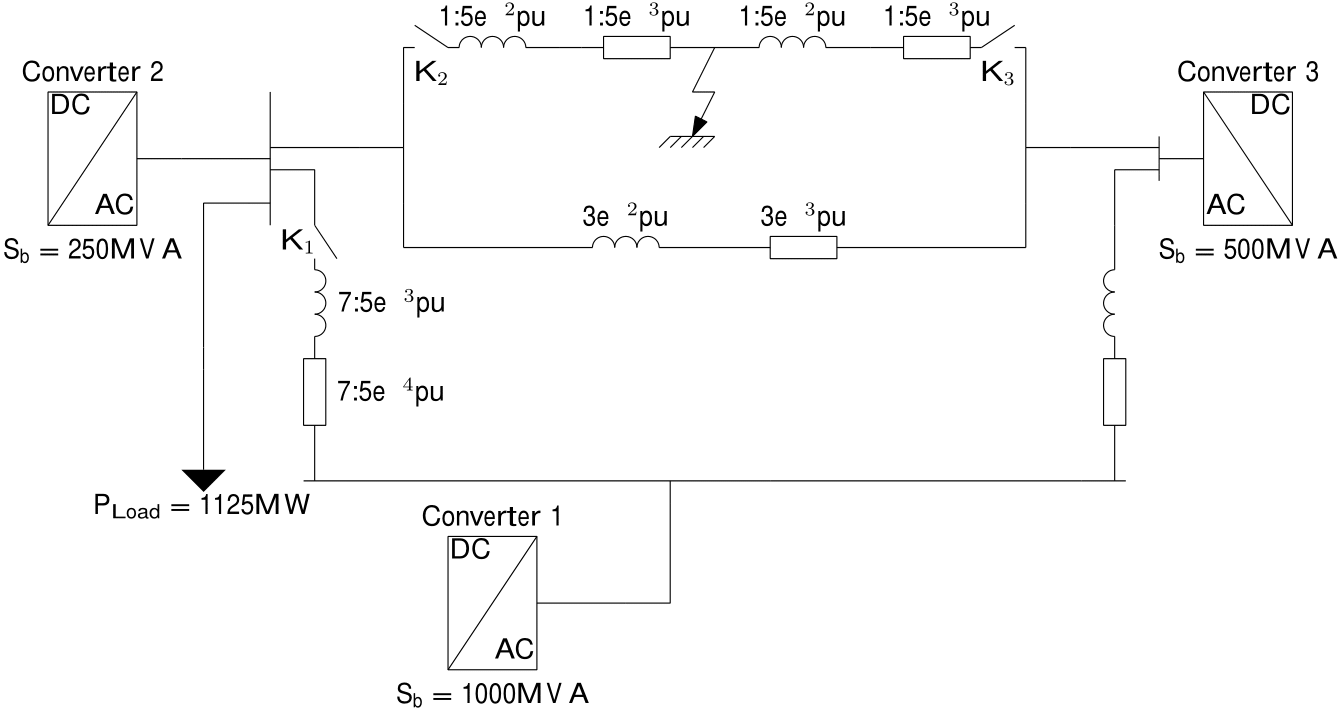
\includegraphics[width=\textwidth]{ThreeConvISGT}
\end{center}
\caption{Structure of the three-converter system\label{ThreeConv}}
\end{figure}
Each converter has a different control: the 1 000 MW converter is using a matching control, the 500 MW a dVOC control and the 250 MW an improved droop control. The network consists in four RL lines, linking together the different converters.
The general structure of the converters and their control is presented in Fig.~\ref{GFGeneral}. The current and voltage loops are common to the three converters while the external loop is different.
\begin{figure}[htbp]
\begin{center}
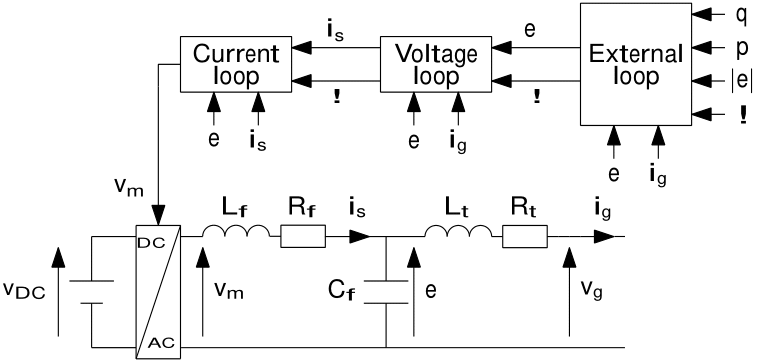
\includegraphics[width=\textwidth]{Schema_Structure_Grid_Forming_and_Control_General}
\end{center}
\caption{Structure of the grid forming converter and its control\label{GFGeneral}}
\end{figure}
Three events are simulated:
\begin{itemize}
\item At $t = 0.5s$, the line connecting the bus 1 and the bus 2 is disconnected ($K_1$ is opened).
\item At $t = 1.5s$, a short-circuit is applied at the middle of the line connecting bus 2 and bus 4.
\item At $t = 1.65s$, the short-circuited line connecting bus 2 and bus 4 is disconnected to clear the fault ($K_2$ and $K_3$ are opened).
\end{itemize}
\section*{Results}
The currents in the three converters during the whole simulation are presented in Fig.~\ref{comp1}.
\begin{figure}[H]
\begin{center}
  \begin{tikzpicture}[scale = 0.8]
    \begin{axis}[grid=major, xmin=0.47, xmax=2.1]
        \addplot[color=blue!50]
        table[x=time,y=Converter250_converter_IConvPu]
        {../reference/outputs/curves/curves.csv};
        \addplot[color=red!50]
        table[x=time,y=Converter500_converter_IConvPu]
        {../reference/outputs/curves/curves.csv};
        \addplot[color=green!50]
        table[x=time,y=Converter1000_converter_IConvPu]
        {../reference/outputs/curves/curves.csv};
        \legend{$i_{c_{Converter250}}$,$i_{c_{Converter500}}$,$i_{c_{Converter1000}}$}
    \end{axis}
  \end{tikzpicture}
  \end{center}
  \caption{Current in the three converters with static lines\label{comp1}}
\end{figure}
All the three controls are stable for this simulation and manage to bring back the current near its set point. During the fault, the current suddenly increases but is then limited thanks to the current limitation that protects the converter from overcurrents.
\par When looking at the frequency of each of the three converter in Fig.~\ref{comp10}, one can see that the frequency is maintained close to $1 pu$ during the whole simulation and that the three converters are well synchronized.
\begin{figure}[H]
\begin{center}
  \begin{tikzpicture}[scale = 0.8]
    \begin{axis}[grid=major, xmin=0.47, xmax=2.1]
        \addplot[color=blue!50]
        table[x=time,y=Converter250_control_omegaPu]
        {../reference/outputs/curves/curves.csv};
        \addplot[color=red!50]
        table[x=time,y=Converter500_control_omegaPu]
        {../reference/outputs/curves/curves.csv};
        \addplot[color=green!50]
        table[x=time,y=Converter1000_control_omegaPu]
        {../reference/outputs/curves/curves.csv};
        \legend{$\omega_{Converter250}$,$\omega_{Converter500}$,$\omega_{Converter1000}$}
    \end{axis}
  \end{tikzpicture}
    \end{center}
  \caption{Frequency of the three converters with static lines\label{comp10}}
\end{figure}
\end{document}
